\documentclass{article}
\usepackage{geometry}
\usepackage{flafter}
\geometry{letterpaper, portrait, margin=1in}

\usepackage{hyperref}
\hypersetup{
    colorlinks=true,
    linkcolor=black,
    filecolor=magenta,
    urlcolor=blue,
}

\usepackage{graphicx}
\graphicspath{ {images/} }

\usepackage{tcolorbox}
\usepackage{textcomp}
\usepackage{gensymb}
\usepackage{indentfirst}

\newcommand{\ans}{$\rule{1.5cm}{0.15mm}$}

\title{RoboJackets Firmware Training Week 2 Lab Guide}
\author{Collin Avidano, Maanas Purushothapu, Arvind Srinivasan}
\date{\today\\v1.0}

\begin{document}
\maketitle{}
\setcounter{tocdepth}{2}
\tableofcontents
\pagebreak

%Everything below is for you to edit. Code above sets up the general formatting for the document

\section{Background}
    \subsection{Topics}
        The important topics being discussed this week in lab include state machines, interrupts, and more complex C++.
    \subsection{Premise}
        The lab premise is to make a state machine that implements a simple counter. This state machine will change states based on the 2 button inputs and will display state using the 5 controllable LEDs.
    \subsection{Interrupt Service Routines}
        Interrupt Service Routines (ISR) are functions that are called when interrupts are activated. These are usually short functions that should be used to update variables in global scope. Remember that interrupts are when your microcontroller gets a signal that makes it stop whats its doing, run the ISR, and then return to the code it was running. Interrupt-based programming is very common for microcontrollers and robots and is usually more efficient that other methods.
        
    \subsection{Simulation}
        If you are using a simulation instead of the hardware, do not worry.  The steps are exactly the same.  Go to the TinkerCad link and you will see the circuit that is a subset of the the hardware. The Arduino you see will be what you use, with the LEDs and buttons replicated as they would be on the actual board. 
        
        \begin{figure}[ht]
            \centering
            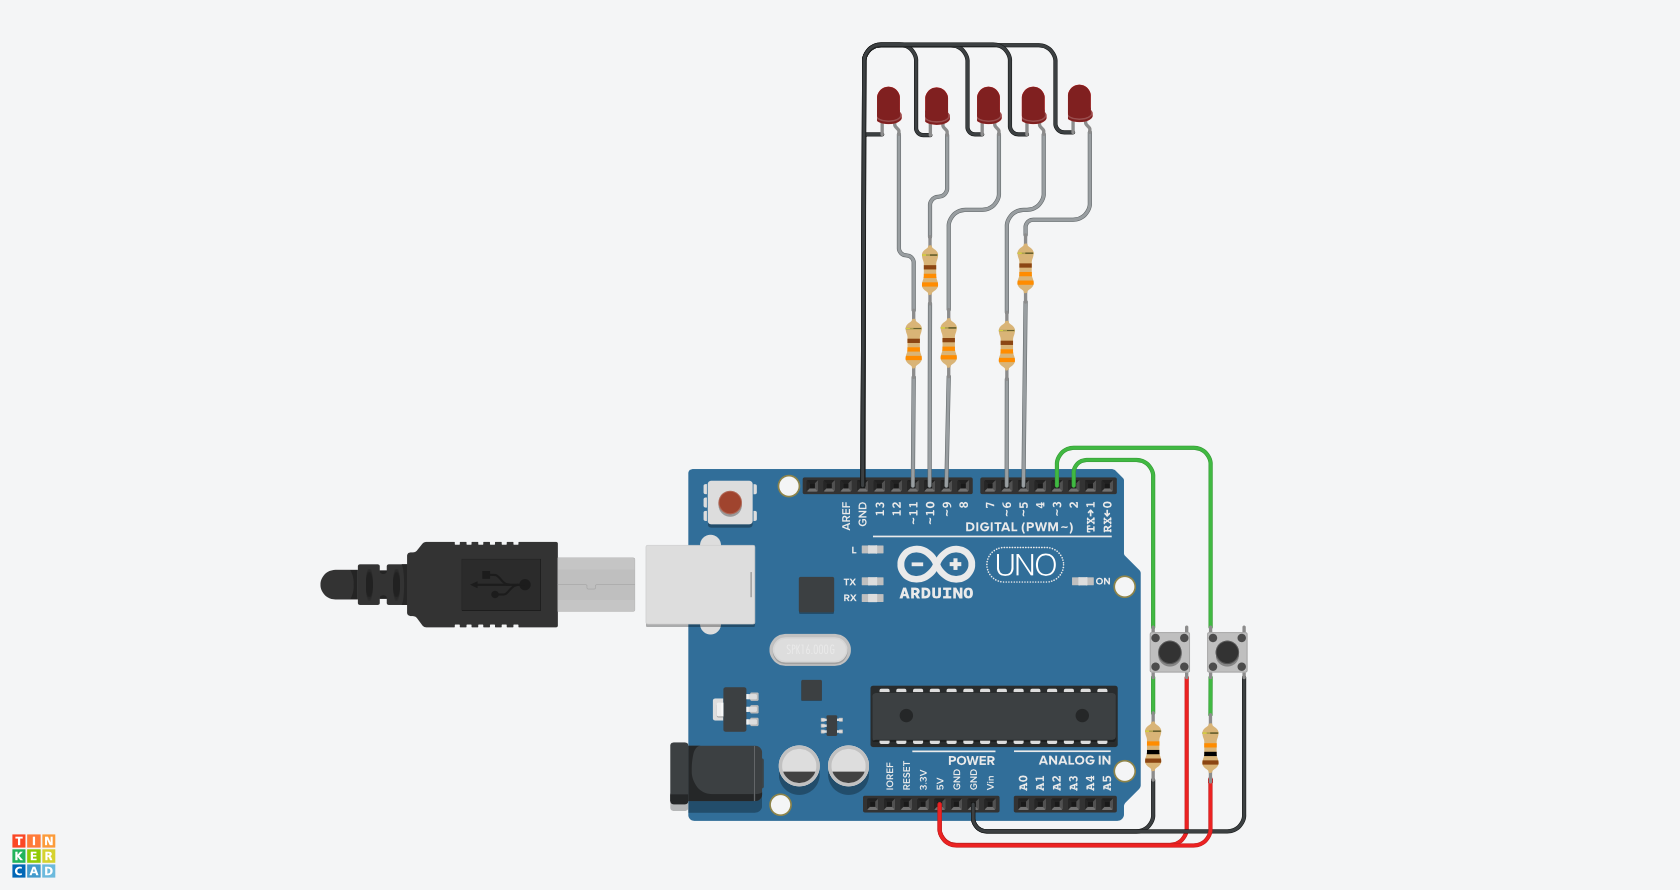
\includegraphics[width = 0.7\textwidth]{images/TinkerCadWires.png}
            \caption{The circuit window of TinkerCAD for this project}
        \end{figure}
        
        \begin{figure}[ht]
            \centering
            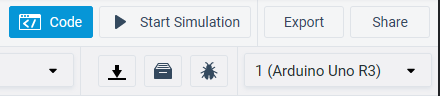
\includegraphics[width = 0.7\textwidth]{images/TinkerCadCode.png}
            \caption{The area which you can use to select your target and compile}
        \end{figure}
        
\section{Materials}
\begin{itemize}
	\item \href{https://www.autodesk.com/education/edu-software/overview}{AutoDesk Education Account}
	\item \href{https://www.tinkercad.com/things/8J1RA4SvqOM}{TinkerCAD}
\end{itemize}
\section{Objectives}
    \subsection{Task 1 - Create State Machine}
        \begin{enumerate}
            \item Plan and draw out the full state machine.
            \begin{itemize}
                \item Make sure you have all the states and transitions marked. 
                \item As a programming convention, we will number our states from 0 upwards, which you will find more useful in the next step.
                \item Don't forget that no LEDs can be on for our counter.
                \item A refresher on state machines can be found in Section \ref{statemachine}.
            \end{itemize}
            \item Write code to display state in \texttt{loop}.
            \begin{itemize}
                \item You will need to go through every LED to set it state, so use a \texttt{for} loop and the \texttt{pinArray} array.
                \item Make sure to use the fact your states are starting counting at 0, which is similar to arrays. 
                \item You will need to use your state variable to know how to do the update.
            \end{itemize}
        \end{enumerate}
    \subsection{Task 2 - Create Interrupts}
        \begin{enumerate}
            \item Write an ISR for each button.
            \begin{itemize}
                \item SW1 is a button that when pressed sends a \texttt{HIGH} value to the Arduino, but is otherwise \texttt{LOW}. You should make sure this button should increase the number of LEDs turned on. 
                \item SW2 is a button that when pressed sends a \texttt{LOW} value to the Arduino, but is otherwise \texttt{HIGH}. This button should decrease the number of LEDs turned on.
            \end{itemize}
            \item Write code in \texttt{setup} for the buttons and interrupts.
            \begin{itemize}
                \item You will also need to setup the buttons as normal digital inputs first. 
                \item Make sure to understand how each button has a different type of change, which will affect how the interrupt triggers.
                \item A refresher on setting up interrupts can be found in Section \ref{attachinterrupt}.
            \end{itemize}
        \end{enumerate}
        
\section{Relevant Information}
    \subsection{State Machines} \label{statemachine}
        State machines are tools to organize the behavior of code, based around a number of "states" or points the code can be at. We specifically are looking at state machines that have output behavior depend only on current state, meaning the number of behaviors equals the number of states. The state machine inputs are used to trigger transitions to different states, with there no transition to an impossible state. A graphical representation is often used with bubbles representing states and labelled arrows representing transitions.
        
        \begin{figure}[ht]
            \centering
            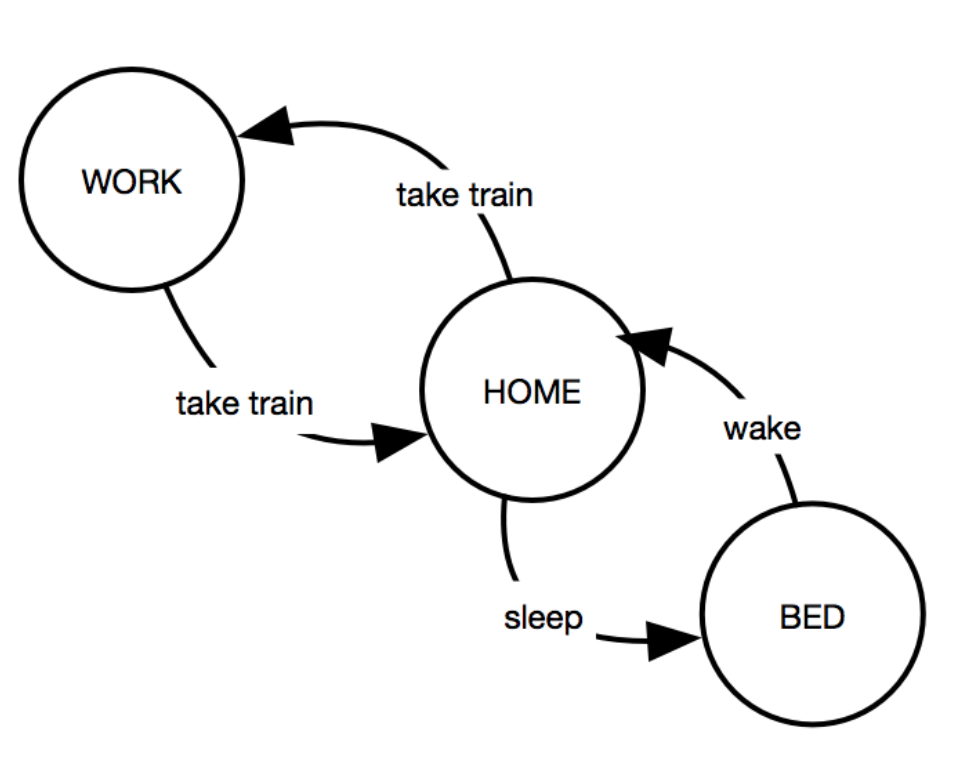
\includegraphics[width = 0.5\textwidth]{images/StateMachine.png}
            \caption{Example State Machine}
        \end{figure}
        
    \subsection{\texttt{attachInterrupt} Function} \label{attachinterrupt}
        The function we will be using for setting up interrupts is the \texttt{attachInterrupt} Function. You can refer to the reference page \href{https://www.arduino.cc/reference/en/language/functions/external-interrupts/attachinterrupt}{here} for understanding it along with examples. Specifically, you need to look into how to convert a pin to a interrupt number and to set the mode that triggers the interrupts.
        
        \begin{figure}[ht]
            \centering
            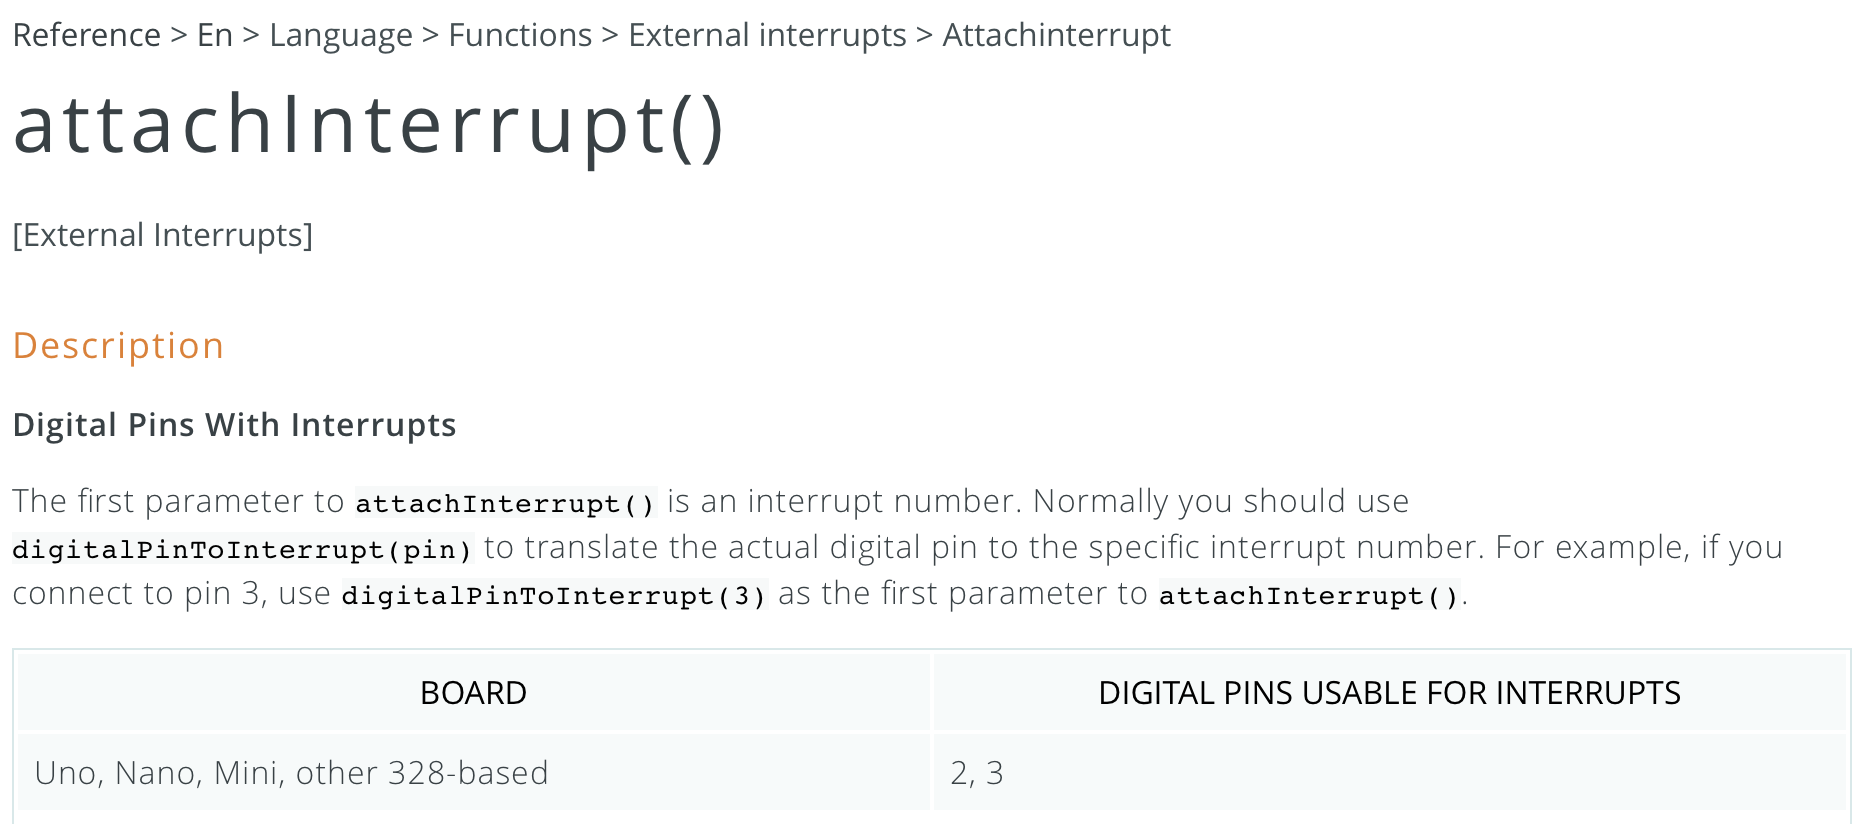
\includegraphics[width = 0.75\textwidth]{images/AttachInterrupt.png}
            \caption{\texttt{attachInterrupt} Function on the Arduino Website}
        \end{figure}
        
\section{Troubleshooting}
    \subsection{Solutions}
    We have included the solutions below if you do not complete the lab during the session or if you want to verify your answer. If you need help during the lab ask an instructor!
\begin{itemize}
    \item \href{https://www.tinkercad.com/things/cGKh5f8nkDv}{TinkerCAD Solution}
    \end{itemize}
\end{document}